\documentclass[main]{subfiles}

\begin{document}

\chapter{Efficient Bessel Decomposition}
\label{chap:EBD}


\paragraph{\bfseries{Abstract}:}We introduce a new algorithm for the fast evaluation of discrete convolutions with radial kernels in $\R^2$ using the Non-Uniform Fast Fourier Transform. In contrast with other approaches, a Fourier representation of the kernel is obtained with frequency samples lying on concentric circles rather than on a Cartesian grid. As a consequence, we require much less terms to reach a given accuracy. This allows for a faster evaluation of the discrete convolution at the cost of longer precomputations. We provide a full analysis of the complexity and error of our method. Numerical results are reported.



\section*{Introduction}

We describe a fast algorithm for computing discrete convolutions of the form

\begin{equation}
q_k = \sum_{l = 1}^{N_z} G(\boldsymbol{z}_k - \boldsymbol{z}_l) f_l\,, \quad k \in \left\{1, \cdots, N_z\right\}\,.
\label{discreteConv}					
\end{equation}
when $G$ is a radial function, i.e. there exists a function $g : \mathbb{R}^+ \to \R$ such that, for almost all $x \in \mathbb{R}^3$, $G(x) = g(|x|)$, where $\abs{\cdot}$ denotes the Euclidean norm. To simplify the notation, we write in such a case $G(x) = G(r)$ where $r = \abs{x}$. We assume that the nodes $\bs{z} = \varInRange{\bs{z}}{k}{1}{N_z}$ lie inside a disk of radius $\rmax$ in $\mathbb{R}^2$. Finally $f = \varInRange{f}{k}{1}{N_z}$ is a complex vector. For example, in the resolution of the Laplace equation with Dirichlet boundary conditions by the boundary integral method with a Krylov one needs to compute many discrete convolutions like Equation \eqref{discreteConv} with $G(\bs{x}) = -\frac{1}{2\pi}\log \abs{\bs{x}}$, the kernel of the single layer potential (when the kernel is singular, we take the convention $G(0) = 0$ in the convolution \eqref{discreteConv}). Their computation are a bottleneck in this method. Discrete convolutions also appear in multiple other fields of mathematics and physics, such as particle simulation, biochemistry, tomography etc.

In principle, the effective computation of the vector $q = (q_k)_{1 \leq k\leq N_z}$ using Equation \eqref{discreteConv} requires $N_z^2$ evaluations of the kernel. However, several more efficient algorithms have emerged to compute an approximation of $q$ with only quasilinear complexity in $N_z$. Among those is the celebrated Fast Multipole Method (FMM, see for example \cite{greengard1988rapid,rokhlin1990rapid, rokhlin1993diagonal, coifman1993fast, cheng1999fast} and references therein). Although this algorithm is very efficient, it suffers from complicated and kernel-specific implementation. For a radial kernel and a 2-dimensional problem, Potts and Steidl \cite{potts2004fast} introduced an algorithm, which we call here \textit{Fastsum}, that is both simpler and more versatile than the FMM, while achieving comparable performances. 

This method relies on the Non-Uniform Fast Fourier Transform (NUFFT, see the seminal paper \cite{NuFFT} and also \cite{greengard2004accelerating,poplau2006calculation,keiner2009using,potts2001fast} and references therein for tutorials, numerical aspects and open source codes) to convert the convolution \eqref{discreteConv} into a product in frequency space. The NUFFT takes as inputs a set of $N_z$ nodes $\bs{z}$ and $N_\xi$ frequency samples $\bs{\xi}$ in $\mathbb{R}^2$, a complex vector $\alpha  \in \mathbb{C}^{N_z}$ and returns the vector  $u \in \mathbb{C}^{N_\xi}$ defined by:
\vspace{-0.1cm}
\[ u_\nu = \sum_{k = 1}^{N_z} e^{\pm i \bs{z}_k \cdot \boldsymbol{\xi}_\nu} \alpha_k\,, \quad \nu \in \left\{1,\cdots,N_\xi \right\}\,.\]
We denote the resulting vector $u$ by $\textup{NUFFT}_{\pm}[z,\xi](\alpha)$. 
This algorithm generalizes the classical Fast Fourier Transform (FFT,  \cite{cooley1965algorithm}) to nonequispaced data, preserving the quasi-linear complexity.

\textit{Fastsum} exploits the NUFFT as follows. A trigonometric representation of the kernel $G$ is derived:
\begin{equation}
\label{Gapprox}
G(\bs{x}) \approx G_{\text{trig}}(\boldsymbol{x}) \isdef \sum_{\nu=1}^{N_\xi} e^{i  \boldsymbol{x}\cdot \boldsymbol{\xi}_\nu} \hat{\omega}_\nu\,,
\end{equation}
where $(\xi_\nu)_{\nu = 1 \cdots N_\xi}$ are the frequency samples in $\R^2$ and $\hat{\omega}_\nu$ are complex numbers. This representation is replaced in \eqref{discreteConv} to yield the fast approximation
\begin{equation}
\begin{split}	q_{k} &\approx \left(\sum_{\nu = 1}^{N_\xi} e^{+i  \bs{z}_k  \cdot\boldsymbol{\xi}_\nu } \left[\hat{\omega}_\nu \sum_{l=1}^{N_z} e^{- i \bs{z}_l \cdot \boldsymbol{\xi}_\nu} f_l) \right]\right)_{1 \leq k \leq N_z}\\
&= \operatorname{NUFFT}_+[\bs{z},\boldsymbol{\xi}]\left(\hat{\omega} \odot \operatorname{NUFFT}_-[\bs{z},\boldsymbol{\xi}]\big(f\big)\right),
\end{split}
\label{far convolution}					
\end{equation}
where $\odot$ denotes the element wise product between vectors.

For 3 space dimensions, an analog method was developed by Alouges and Aussal, named the Sparse Cardinal Sine Decomposition (SCSD). The main difference lies in the choice of the frequency samples in the representation \eqref{Gapprox}. Instead of choosing them on a Cartesian grid like \textit{Fastsum}, the SCSD allows for nonequispaced frequencies and seeks a trigonometric representation with the smallest possible number of terms. This non-linear and high-dimensional minimization problem is made tractable by exploiting the radial symmetry of the problem. 

The aim of this work is to adapt the SCSD method to 2 space dimensions. The cardinal sines must be replaced by Bessel functions and the frequencies are chosen on a set of concentric circles centered at the origin. We obtain trigonometric representations with much fewer terms than in \textit{Fastsum}. Since the frequencies are no longer equispaced, the slower NUFFT of type 3 must be used instead of type 1 (following the terminology of \cite{lee2005type}). Nevertheless, the numerical tests, exposed in \autoref{sec:numericalPerf}, show that the gain in number of frequency samples leads to a faster evaluation of \eqref{discreteConv}, at the cost of longer precomputations.

The remainder of the paper is organized as follows. We first give a self-contained description of our algorithm in \autoref{sec:overview}, and state its complexity in \autoref{The:GlobalComplexity} in a special case. Then, \autoref{sec:FourierBesselSeries} briefly presents the theory of Fourier-Bessel decomposition. In \autoref{sec:EBD}, we analyze the "Efficient Bessel Decomposition" (EBD), a new method to approximate singular kernels by Bessel series outside the origin with only a small number of terms. In \autoref{sec:ApplicationLaplaceHelmholtz}, we estimate the number of terms required in the EBD to reach a given accuracy for the logarithmic kernel. We also describe how to deal with other kernels. In \autoref{sec:circular}, we show how to convert a Bessel decomposition into a trigonometric polynomial through what we call "circular quadratures". In \autoref{sec:complexities}, we summarize the complexity of each step and prove \autoref{The:GlobalComplexity}. We finally give a numerical comparison of our algorithm with \textit{Fastsum}. 

A Matlab code of the method described here is available online \cite{EBD}. 


\section{Summary of the algorithm}

\setcounter{equation}{0}
\numberwithin{equation}{section} % Numérote les équations section.numéro.
\label{sec:overview}

\subsection{Trigonometric representation}

In this section, given a cut-off parameter $\rmin > 0$ (also recall $\rmax$ is the diameter of the set of nodes $z$), we describe how to select the frequency samples $(\xi_\nu)$ in the trigonometric representation \eqref{Gapprox}.

\paragraph{Efficient Bessel Decomposition.} 

We first reduce to a $1$-dimensional approximation problem. We find a linear combination of Bessel functions approximating $G(r)$ on $[\rmin,\rmax]$:
\begin{equation}
G(r) \approx G(\rmax) + \sum_{p=1}^P \alpha_p J_0\left(\rho_p \frac{r}{\rmax}\right)\,, \quad r \in [\rmin,\rmax]\,,\label{decompRadiale}
\end{equation}
where $J_0$ is the Bessel function of first kind and zero order and $(\rho_p)$ is the sequence of its roots (see \autoref{defJ0} for more details). We choose $\alpha_1,\cdots, \alpha_{P}$ as the minimizers of the least square error
\[E(\alpha_1,\cdots,\alpha_P) = \bigintsss_{\rmin}^{\rmax}r \left[\frac{d}{dr}\left(G(r) - \sum_{p=1}^P \alpha_p J_0\left(\rho_p \frac {r}{\rmax}\right)\right)\right]^2 dr\,.\]
The number of terms $P$ is chosen as the smallest integer for which the $L^\infty$ error is below a given tolerance. This amounts to solving a series of linear systems where the matrix coefficients are explicit (see \autoref{epEstUneBaseDeHilbert}). The right-hand side can be approximated by numerical quadrature when an explicit formula is not available. In \autoref{sub:NumStab}, we show how to compute the vector $(\alpha_p)$ with the minimal length without solving a full linear system for each candidate $P$.   
\paragraph{Circular quadrature.}In a second step, we write for each $p \in \{ 1,\cdots, P \}$
\begin{equation}
J_0(\rho_p \abs{\bs{x}}) \approx \dfrac{1}{M_p}\sum_{m=0}^{M_p-1}e^{i \rho_p \bs{\xi}_p^m \cdot \bs{x}}\,,
\label{DecompJ0_p}
\end{equation}
where $\xi^m_p = \left(\cos\left(\frac{2\pi m}{M_p}\right),\sin\left(\frac{2\pi m}{M_p}\right)\right)$. This is the trapezoidal rule applied to the identity
\[ J_0(\rho_p\abs{\bs{x}}) = \frac{1}{2\pi}\int_{\abs{\bs{\xi}}=1}{e^{i \rho_p\bs{x} \cdot \bs{\xi}}} d\sigma(\bs{\xi})\,.\]
The trigonometric representation \eqref{Gapprox} is obtained by combining Equations \eqref{decompRadiale} and \eqref{DecompJ0_p}. A criterion for choosing the number of terms $M_p$ is derived in \autoref{sec:circular}.  


\subsection{Description of the algorithm and complexity}
\label{fullDescr}
The full algorithm is split into two parts:

\paragraph{Offline part.}
\begin{itemize}
	\item[]\textbf{Inputs:} A radial kernel $G$, a set of $N_z$ nodes $\bs{z}$ in $\mathbb{R}^2$ of diameter $\rmax$, a cut-off parameter $\rmin$ and a tolerance $\varepsilon > 0$.
	\item[]\textbf{Trigonometric representation:} Combine the Bessel decomposition and the circular quadrature to obtain the trigonometric representation $G_\text{trig}$ of $G$, as in Equation \eqref{Gapprox}. This approximation is valid for $\rmin \leq r\leq \rmax$ up to the tolerance $\varepsilon$. 
	\item[]\textbf{Correction Matrix:} Determine the set $\mathcal{P}$ of all the pairs $(k,l)$ such that $\abs{\bs{z}_k - \bs{z}_l} \leq \delta_{\min}$ (fixed-radius neighbor search). Assemble the close correction sparse matrix:
	\begin{equation}
	\label{defD}
	D_{kl} = \delta_{(k,l) \in \mathcal{P}} \left( G({\bs{z}_k - \bs{z}_l}) - G(\rmax) - \sum_{p = 1}^{P} \alpha_p J_0\left(\rho_p\frac{\abs{z_k - z_l}}{\rmax}\right)\right).
	\end{equation}
	The last two terms inside the parentheses counteract the error introduced by the approximation of $G$ in Bessel series near the origin. The last sum is computed efficiently using a piecewise polynomial interpolation of the function 
	\[ r\mapsto \sum_{p = 1}^{P} \alpha_p J_0\left(\rho_pr\right),\quad r \in \left(0,\rmin\right). \]
	\item[] \textbf{Outputs}: The set of weights $(\hat{\omega}_\nu)$, the frequency samples $(\boldsymbol{\xi}_\nu)$ and the (sparse) correction  matrix $D$. 
\end{itemize}
\paragraph{Online part.}
\begin{itemize}
	\item[] \textbf{Inputs:} We take in input all outputs of the offline part, and a complex vector $f$ of size $N_z$. 
	\item[] \textbf{Far approximation:} Compute
	\begin{equation}
	\label{FarApprox}
	q^{\text{far}}_k = \sum_{l=1}^{N_z} G_{\textup{trig}}(\bs{z}_k - \bs{z}_l) f_l, \quad 1 \leq k \leq N_z
	\end{equation} 
	in the following three steps:
	\begin{itemize}
		\setlength{\itemindent}{2em}
		\item[(i)] \textbf{Space $\rightarrow$ Fourier: } Compute $\hat{f} = \textup{NUFFT}_-[\bs{z},\boldsymbol{\xi}](f).$
		\item[(ii)] \textbf{Fourier multiply:} Perform an element-wise multiplication by $\hat{\omega}$:
		\[{\hat{g}_{\nu} \isdef \hat{\omega}_\nu \hat{f_\nu}.}\]
		\item[(iii)] \textbf{Fourier $\rightarrow$ Space: } Compute $q^{\text{far}} =  \textup{NUFFT}_+[\bs{z},\boldsymbol{\xi}](\hat{g}).$
		\setlength{\itemindent}{0em}
	\end{itemize}
	
	\item[] \textbf{Close correction:} Compute the sparse matrix product:
	\[q^{\textup{close}} = Df \,.\]
	\item[] \textbf{Output:} The vector $q = q^{\textup{far}} + q^{\textup{close}}$, with, for any $k \in \left\{1,\cdots,N_z\right\},$	
	\[ \abs{q_k - \sum_{l = 1}^{N_z} G({\bs{z}_k - \bs{z}_l}) f_l} \leq \varepsilon \sum_{l=1}^{N_z} \abs{f_l}\,.\]
\end{itemize}
For the special case of the logarithmic kernel and for nodes uniformly distributed on a curve, the complexity of the algorithm is given by the following theorem, which is proved in \autoref{sec:complexities}.
\begin{theorem} Assume the nodes $(\bs{z}_k)$ are uniformly distributed on a regular curve, and $G(\bs{x}) = \log \abs{\bs{x}}$. Let $\varepsilon > 0$ the desired accuracy of the method. Let 
	\[a =\dfrac{1}{N_z^{2/3 - \eta}}\]
	for some $\eta \in \left[0,\frac{1}{6}\right]$, and choose 
	\[\rmin = a \rmax \,.\] 
	Then there exists a constant $C>0$ independent of $N_z$, $\varepsilon$ and $\eta$ such that:
	\label{The:GlobalComplexity}
	\begin{itemize}
		\item[(i)] The number of operations required for the computation of the trigonometric representation \eqref{Gapprox} valid for $\abs{\bs{x}} \in [\rmin,\rmax]$  is bounded by 
		\[ C_{\textup{off}}(N_z,\varepsilon,\eta) \leq C \abs{\log \varepsilon}^3 N_z^{2 - 3\eta}\,,\]
		\item[(ii)] The number of operations required for the assembling of the close correction matrix $D$ is bounded by
		\[C_{\textup{assemble}}(N_z,\varepsilon,\eta)\leq C  N_z^{4/3 + \eta}\,,\]
		\item[(iii)] Once these two steps have been completed, the discrete convolution \eqref{discreteConv} can be evaluated for any choice of vector $f$ at a precision at least $\varepsilon \displaystyle\sum_l \abs{f_l}$ in a number of operations bounded by
		\[C_{\textup{on}}(N_z,\varepsilon,\eta) \leq C \left(  N_z ^{4/3 + \eta} + N_z^{4/3 - 2\eta} \log(N_z) \abs{\log \varepsilon}^4 \right).\] 
	\end{itemize} 
\end{theorem}

The choice for the parameter $a$ depends on the distribution of nodes $z$. For example, for data uniformly distributed on a disk, if we choose $a \propto \frac{1}{\sqrt{N_z}}$ we obtain complexities of $O(\abs{\log \varepsilon}^3  N_z^{3/2})$ and $O(\abs{\log \varepsilon}^4 N_z\log(N_z))$ for the offline and online parts respectively. 



\section{Series of Bessel functions and error estimates}
\label{sec:FourierBesselSeries}
In this section, we give a short introduction to Fourier-Bessel series as an orthonormal decomposition on the eigenfunctions of the Laplace operator, and study the truncation error for smooth functions. We suggest \cite{abramowitz1964handbook,NIST:DLMF} and \cite[chap. 18]{watson1995treatise} for background. The main result needed for our purpose is \autoref{DecroissanceFourierBessel}. 

Our method can be adapted for any space dimension. For example, in $\R^3$ the radial eigenvalues of the Laplace operator are proportional to
\[  \bs{x} \mapsto \dfrac{J_{1/2}(2\pi p\abs{\bs{x}})}{\bs{|x|}^{1/2}}, \quad  p\in\N^*.\] 
In other words, our approach generalizes \cite{Alouges2015} to any dimension.  
\subsection{Radial eigenfunctions of Laplace's operator with Dirichlet boundary conditions}
\label{FunctionalFramework}
In the following, $B$ denotes the unit ball in $\mathbb{R}^2$ and $\partial B$ its boundary. Let $\Lrad$ the space of those functions in $L^2(B)$ that are radial and 
$$\Crad = \enstq{\varphi \in \Cinf_c(B)}{\varphi \text{ is radial }}\,.$$
Similarly, let $\Hrad = H^1(B) \cap \Lrad$, where $H^1(B)$ is the usual Sobolev space of square integrable functions with square integrable weak derivatives. $\Hrad$ is a Hilbert space for the norm
\[\norm{u}_{\Hrad}^2 = \int_{B}\abs{u(x)}^2 + \abs{\nabla u(x)}^2dx = 2\pi\int_{0}^1 r \left(u(r)^2 + u'(r)^2\right) dr \,. \]
Finally, $\Hzrad$ is the closure of $\Crad$ in $\Hrad$, with the equivalent norm
\[\norm{u}_{\Hzrad}^2 = {2\pi \int_{0}^1 r u'(r)^2dr}\,.\] 
\noindent We now briefly recall some facts on Bessel functions. 
\begin{definition}
	\label{defJ0}
	The Bessel function of the first kind and order $\alpha$, $J_\alpha$ is defined by the power series: 
	\begin{equation}
	\label{J0powerSeries}
	J_\alpha(r) \isdef \sum_{m=0}^\infty \frac{(-1)^m}{m! \, \Gamma(m+1+\alpha)} {\bigg(\frac{r}{2}\bigg)}^{2m+\alpha}\!\!\!\!\!\!\!\!\!\!\!\! \,.
	\end{equation}
\end{definition}
The roots $(\rho_p)_{p \in \N^*}$ of $J_0$, behave for large $p$ as 
\[ \rho_p \underset{p \to \infty}{\sim} \pi p\,.\]

\noindent For any $p\in \N^*$, we introduce:
\[e_p(\bs{x}) = C_p J_0(\rho_p \abs{\bs{x}})\,,\]
where the normalization constant $C_p$ is chosen such that $\norm{e_p}_{H^1_0(B)} = 1$, that is  
\[C_p = \dfrac{1}{\left(2\pi \int_B  r \rho_p^2 J_1 (\rho_p r)^2\right)^{1/2}} = \dfrac{1}{\sqrt{\pi}\rho_p\abs{J_1(\rho_p)}}\,.\]
One can check, using asymptotic expansions of Bessel functions, (see for example equations  (10.17.1 - 10.17.3) in \cite{NIST:DLMF}) that
\begin{equation}
\label{estimCp}
C_p = \dfrac{1}{\sqrt{2 \pi p}} + O\left(\frac{1}{p^{3/2}}\right)\,, 
\end{equation}
\noindent For any $p \in \N^*$, $e_p$ satisfies:
\begin{equation}
\label{epEstUnVP}
-\Delta e_p = \rho_p^2 e_p\,.
\end{equation}
In the sequel, we denote by $\mathcal{A}(a)$ the annulus 
\[\mathcal{A}(a) = \enstq{x\in \R^2}{\abs{x} \leq a}\,.\]
\begin{theorem} 
	\label{epEstUneBaseDeHilbert}
	The family $\left\{e_p \mid p\in \N^*\right\}$ is a Hilbert basis of $\Hzrad$. For $0 \leq a \leq 1$, the $H^1_0$ scalar product on the annulus $\mathcal{A}(a)$ of two eigenfunctions is given by the following formulae:
	\[ \int_{\mathcal{A}(a) } \nabla e_i \cdot \nabla e_j = \frac{2\pi C_i C_j \rho_i \rho_j}{\rho_j^2 - \rho_i^2}\bigg[F_{i,j}(1) - F_{j,i}(1) - F_{i,j}(a) + F_{j,i}(a)\bigg]\]
	if $i \neq j$, 
	where 
	\[	 F_{i,j}(r) =  \rho_i r J_0(\rho_i r)J_0'(\rho_j r)\,,\]
	while
	\begin{equation*}
	\int_{\mathcal{A}(a) } \abs{ \nabla e_i}^2 = 2\pi C_i^2 \big(F_i(1) - F_i(a)\big)
	\end{equation*}
	where 
	\[F_i(r) = \rho_i^2r^2\left[\dfrac{1}{2}J_0(\rho_ir)^2 + \frac{1}{2}J_0'(\rho_ir)^2\right] + \rho_irJ_0(\rho_i r)J_0'(\rho_ir)\,.\]
\end{theorem}
\begin{proof}
	The Laplace operator is self-adjoint, positive definite on $H_0^1(B)$ thus its normalized eigenfunctions form a Hilbert basis of this space. Their expression is given in \cite[Eq. (3.9)]{grebenkov2013geometrical} in polar coordinates $(r,\varphi)$ by
	\[u_{nkl}(r,\varphi) = J_n(j_{nk}r ) \begin{cases}
	\cos(n\varphi) & l = 1,\\
	\sin(n\varphi) & l = 2 \text{ } (n \neq 0)\,.
	\end{cases}\]
	where $j_{nk}$ is the $k$-th positive root of $J_n$. The fact that $(e_p)$ is a Hilbert basis of $\Hzrad$ stems from the observation that the radial functions are $H^1_0$ orthogonal to $u_{nkl}$ as soon as $n \neq 0$. The scalar product formulae can be verified by differentiating the functions $F_{i,j}$ and $F_i$. 
	
\end{proof}
\subsection{Truncation error for smooth functions}
\label{FourierBesselTruncError}
We now present the Fourier-Bessel series and prove a bound for the truncation error. First of all, \autoref{epEstUneBaseDeHilbert} implies that any function $f \in \Hzrad$ can be expanded through its so-called Fourier-Bessel series as
\[f = \sum_{p\in \mathbb{N}^*}c_p(f)e_{p}\,,\]
where the "Fourier-Bessel" coefficients $c_p(f)$ are given by
\[c_p(f) = \displaystyle \int_B \nabla f(\bs{x}) \cdot \nabla e_{p}(\bs{x}) d\bs{x} = \rho_p ^2 C_p\int_{0}^1 r f(r) J_0(\rho_p r) dr\,.\]
See for example \cite[Chap. 18, Eq. (2)]{watson1995treatise}. Notice the second equality is obtained by integration by part. We will show that the coefficients decay rapidly when $f$ is smooth. To this aim, we first introduce the following terminology: 
\begin{definition}
	A radial function $f$ satisfies the multi-Dirichlet condition of order $n \in \N^*$ if $f$ is $H^{2n}$ in a neighborhood of $\partial B$ and if for all $s \leq n-1$, the $s$-th iterate of $-\Delta$ on $f$, $(-\Delta)^s f$, vanishes on $\partial B$ (with the convention $(-\Delta)^0 f = f$). 
\end{definition}
An equivalent statement of the following result can be found in \cite[Chap. 8, Sec. 20, Thm. 1]{tolstov2012fourier}. The proof is reproduced here for the reader's convenience. 
\begin{proposition} 
	\label{DecroissanceFourierBessel}
	If $f \in H^{2n}(B)$ satisfies the multi-Dirichlet condition of order $n$, then for any $p \in \mathbb{N}^*$:
	\[ c_p(f) = \dfrac{1}{\rho_{p}^{2n-2}} \int_{B}\left(-\Delta\right)^{n} f(\bs{x})e_p(\bs{x}) d\bs{x}\,.\] 
\end{proposition}
\begin{proof}
	We show this by induction. Let $f$ satisfy the multi-Dirichlet condition of order $n=1$, then by integration by parts:
	\[c_p(f) = \int_{B}(-\Delta)f(\bs{x}) e_p(\bs{x})d\bs{x}\,,\]
	since $e_p$ vanishes on $\partial B$.
	Assume the result is true for some $n \geq 1$ and let $f$ satisfy the multi-Dirichlet condition of order $n+1$. Then, using $-\Delta e_p = \rho_p^2e_p$, we get
	\[c_p(f) = \frac{1}{\rho_p^{2n}}\int_{B}(-\Delta)^{n}f(\bs{x})~ (-\Delta) e_p(\bs{x}) d\bs{x}\,.\]
	The result follows from integration by parts where we successively use that $(-\Delta)^{n}f$ and $e_p$ vanish on $\partial B$.
	
\end{proof}

\begin{corollary} Let the remainder be defined as 
	\[R_P(f) = \displaystyle\sum_{p = P+1}^{+\infty} c_{p}(f) e_{p}\,.\]
	If $f \in H^{2n}(B)$ satisfies the multi-Dirichlet condition of order $n$, there exists a constant $C$ independent of $n$ and $P$ such that: 
	\[\norm{R_P(f)}_{H^1_0(B)} \leq C\dfrac{\norm{(-\Delta)^n f}_{L^2(B)}}{(\pi P)^{2n}}\sqrt{\dfrac{P^3}{n}}\,.\]
	\label{EstimationRest}
\end{corollary}																												
\begin{proof}
	Parseval's identity yields $\norm{R_P(f)}_{\Hzrad}^2 = \sum_{p=P+1}^{+\infty}|c_p(f)|^2.$
	By \autoref{DecroissanceFourierBessel} and using $\rho_p \sim \pi p$, we can find a constant $C$ such that $\abs{c_p(f)} \leq C \frac{\norm{(-\Delta)^n f}_{L^2}}{(\pi p)^{2n - 1}}$. Thus, 
	\[\norm{R_P(f)}_{\Hzrad} \leq C \norm{(-\Delta)^n f}_{\Lrad}\sqrt{\sum_{p= P+1}^{+\infty} \dfrac{1}{(\pi p)^{4n-2}}}\,.\]
	The announced result follows from $\displaystyle\sum_{p > P} \frac{1}{p^{\alpha}} \propto \frac{1}{(\alpha - 1)P^{\alpha-1}}$ for $\alpha > 1$. 
\end{proof}


\subsection{Other boundary conditions}
\label{Robin}
When we replace the Dirichlet boundary condition by the following Robin boundary conditions
\begin{equation}
\label{robinCondition}
\dfrac{\partial u}{\partial n} + H u = 0
\end{equation}
for some constant $H \geq 0$, the same analysis can be conducted, leading to Dini series (also covered in \cite{watson1995treatise}). This time, we construct a Hilbert basis of $\Hrad$ with respect to the bilinear form
\[a_H(u,v) \isdef \int_{B} \nabla u(\bs{x} ) \cdot \nabla v(\bs{x} ) d\bs{x} + H \int_{\partial B}{u(\bs{x} )v(\bs{x} )}d\sigma(\bs{x} ).\]
The following result holds. 
\begin{theorem}
	Let $(\rho_p^H)_{p \in \N*}$ the sequence of positive solutions of
	\[r J_0'(r) + H J_0(r) = 0.\]
	\begin{itemize}
		\item[(i)] If $H>0$, the functions 
		\[e_p^H(r) = C_p J_0(\rho_p^H r),\]
		with $C_p$ such that $a_H(e_p^H,e_p^H) = 1$, form a Hilbert basis of $H^1_{\text{rad}}(B)$. 
		\item[(ii)]If $H = 0$, a constant function must be added to the previous family to form a complete set. 
	\end{itemize}
\end{theorem}
\noindent The truncation error estimates in \autoref{EstimationRest} can be generalized to functions satisfying multi-Robin conditions of order $n \geq 1$, that is for all $s\leq n-1$, $(-\Delta)^s u$ satisfies \eqref{robinCondition}.



\section{Efficient Bessel Decomposition}
\label{sec:EBD}		
In this section, we describe the method for approximating a singular function outside the origin by a Fourier-Bessel series with only a few terms. 
\subsection{Definition}
\label{sub:defEBD}					
Consider the kernel $G$ involved in \eqref{discreteConv}. We can assume up to rescaling $G$ that the diameter $\rmax$ of the nodes $\bs{z}$ is $1$, and therefore, we need to approximate the kernel only on the unit ball $B$. To apply the previous results, two kinds of complications may arise:
\begin{itemize}
	\item[(i)] When $G$ is singular near the origin, it is not in $H^{2n}(B)$ (even for $n=1$). 
	\item[(ii)] The multi-Dirichlet conditions may not be fulfilled up to a sufficient order.
\end{itemize}

The point (ii) is crucial in order to apply the error estimates of the previous section. The first two kernels that we will study (Laplace and Helmholtz) in the next section satisfy the favorable property:
\[\Delta G = \lambda G\]
for some $\lambda \in \mathbb{C}$, is helpful to ensure (ii) at any order. For more general kernels, we suggest a simple trick to enforce multi-Dirichlet conditions up to a given order in \autoref{begal1}. 

First, we deal with point (i). We avoid the singularity by approximating $G$ only in the annulus $\mathcal{A}(a)$. We look for coefficients $(\alpha_p)$ such that
\begin{equation}
G(r) \approx \sum_{p = 1}^P \alpha_p e_p(r), \quad  a< r < 1
\label{temp2}
\end{equation}
for some $P>0$, where we remind the reader that $e_p$ are the radial eigenvalues of the Laplace operator on the unit ball defined in \autoref{sec:FourierBesselSeries}. We call this the Efficient Bessel Decomposition (EBD) of $G$. The EBD coefficients are chosen as the minimizers of the $H^1_0$ error on the annulus $\mathcal{A}(a)$:
\[ E(\alpha_1,\alpha_2,...,\alpha_P) = \bigintsss_{\mathcal{A}(a)} \left|\nabla \!\left( G(\bs{x}) - \sum_{p=1}^P \alpha_p e_p(x)\right)\right|^2d\bs{x}.\] 
Given a tolerance $\varepsilon$, we choose $P$ as the smallest integer for which the $L^\infty$ error of the approximation is below $\varepsilon$. Clearly, for any radial extension $\tilde{G}$ outside the annulus $\mathcal{A}(a)$, one has 
\begin{equation}
E(\alpha_1,\cdots,\alpha_P) \leq \norm{\tilde{G} - \sum_{p = 1}^P c_p(\tilde{G})e_p(x)}^2_{H^1_0(B)}
\label{estimParProlongement}
\end{equation}
In particular, when $\tilde{G}$ is smooth up to the origin, this gives an immediate error estimate via \autoref{EstimationRest}. 
\begin{remark}
	\label{RemarkPotts}
	In \textit{Fastsum}, an explicit polynomial regularization and periodisation $\tilde{G}$ is constructed and the function $G$ is replaced by the discrete Fourier expansion of $\tilde{G}$. In contrast here, the way we choose the coefficients $\alpha_p$ ensures that we get less terms than if we had constructed any particular extension $\tilde{G}$ and used $\alpha_p = c_p(\tilde{G})$. 
\end{remark}
\begin{remark}
	\label{RemLinf}
	In our context, the $H_0^1$ error controls the $L^{\infty}$ norm on $\mathcal{A}(a)$, thus ruling out any risk of Gibb's phenomenon. Indeed, for a function $u$ that vanishes on $\partial B$, one has
	\[\abs{u(\bs{x}_0)} \leq \sqrt{\dfrac{-\log \abs{\bs{x}_0}}{2\pi}}\sqrt{\int_{\mathcal{A}(a)} \abs{\nabla u(\bs{x})}^2} d\bs{x},\quad  \text{almost for all }\bs{x}_0 \in \mathcal{A}(a),\]
	as can be shown by applying the Cauchy-Schwarz inequality to $u(r) = -\int_{r}^{1} u'(t)dt.$
\end{remark}	


\subsection{Numerical computation of the EBD}
\label{sub:NumStab}

\paragraph{Efficient computation of the coefficients.}					
For a given kernel $G$ and integer $P >0$, the EBD coefficients $\alpha_1,\cdots,\alpha_P$ are found by solving the following linear system: 
\begin{equation}
\begin{split}
\sum_{q = 1}^P \rho_q C_q\left(\int_{\mathcal{A}(a)} J_1(\rho_p|\bs{x}|)  J_1(\rho_q|\bs{x}|) d\bs{x}\right) \alpha_q \\
\quad = -\int_{\mathcal{A}(a)} G'(\bs{x}) J_1(\rho_p|\bs{x}|)d\bs{x}, \quad 1\leq p \leq P,
\end{split}	
\label{LinearSystem}
\end{equation}
where $J_1$ is the Bessel function of first kind and order $1$ (in fact, $J_0' = - J_1$). The explicit matrix entries are given in \autoref{epEstUneBaseDeHilbert}. 

Using Cholesky decomposition, it is possible to compute efficiently the solution of the system for $P'$ coefficients from the solution for a greater $P$. Indeed, for $P \in \N^*$, let us call $A_P$ the system matrix and $b_P$ the second member. If $C_P$ is the first Cholesky factor, then $C_{P'}$ is obtained by extracting the top left $P'\times P'$ sub-matrix of $C_P$. Moreover, $b_{P'}$ is just the vector formed of the first $P'$ entries of $b_P$. This way, once the tolerance is reached, we can efficiently remove as many terms as possible. 
\newcommand{\Pa}{\gamma}

\paragraph{Numerical stability.}	

Numerical evidence strongly suggests that the conditioning number ($\text{cond}_2$) of the linear system \eqref{LinearSystem} only depends on the parameter $\Pa \isdef Pa$. This is shown in \autoref{isoValues} where we plot the isovalues of the condition number of the system in function of $P$ and $\gamma$. One can observe the condition number is almost insensitive to the value of $P$ for constant $\gamma$. 

\begin{figure}[t]
	\centering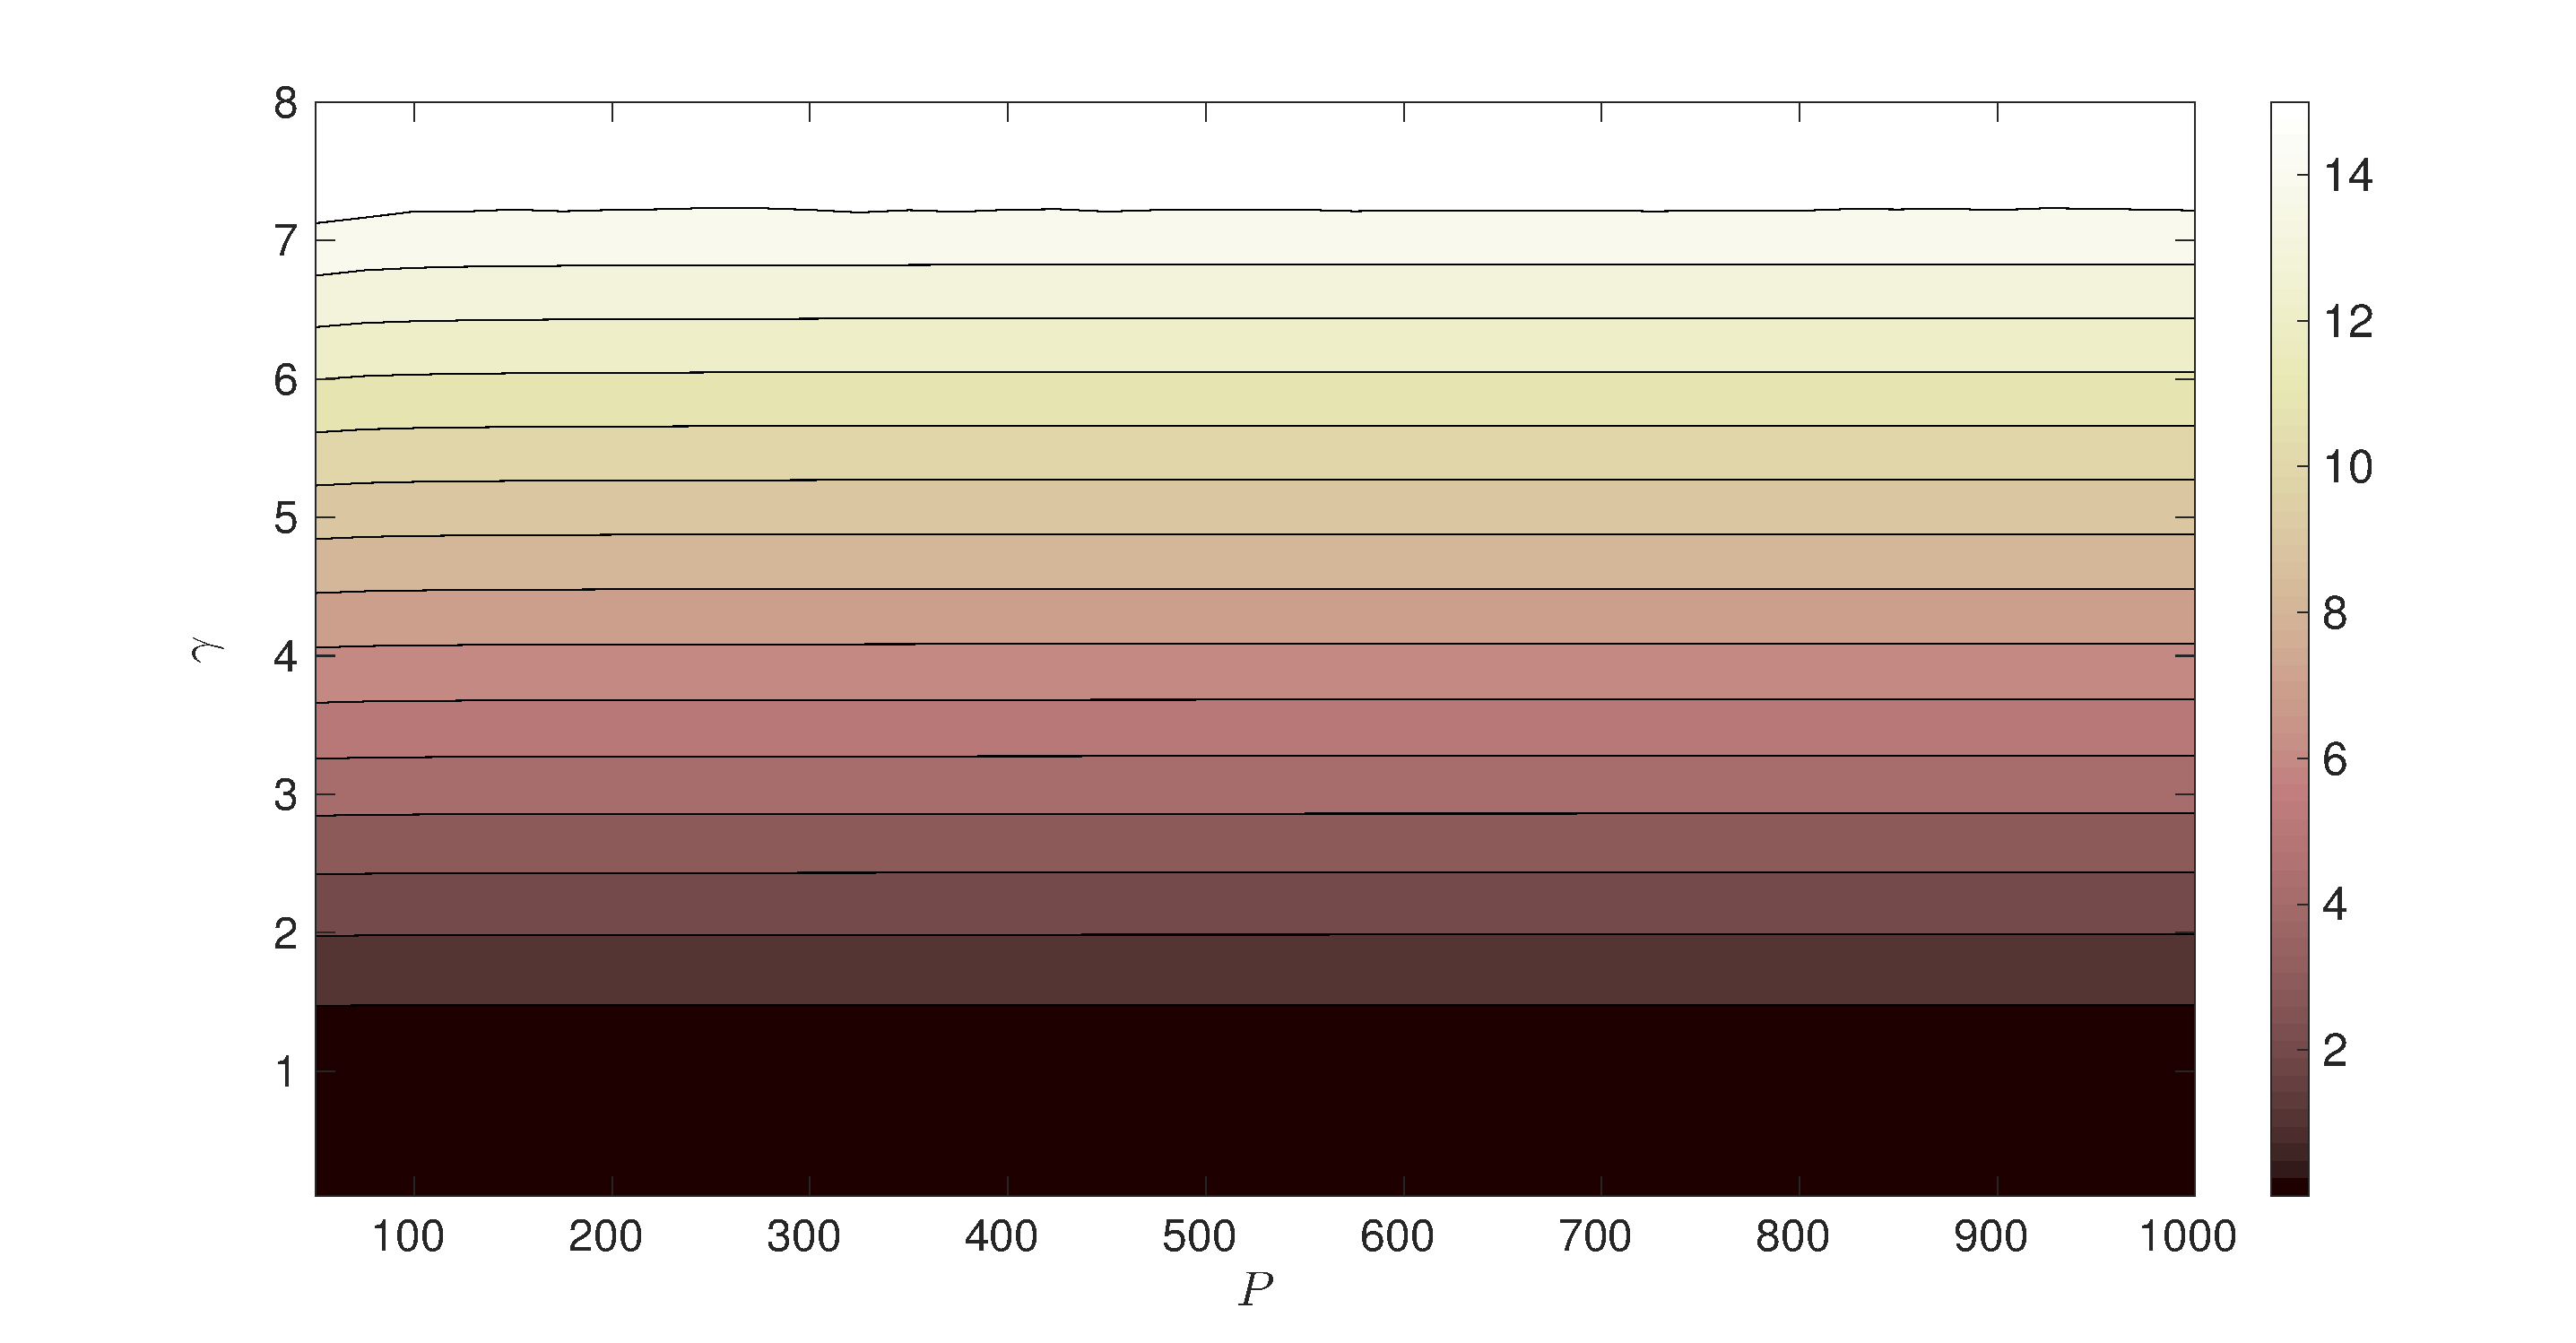
\includegraphics[scale = 0.15]{EBD/figs/isoValues-eps-converted-to}
	\caption{Isovalues of the function $(P,\gamma) \mapsto \log_{10} (\text{cond}_2(A))$ where $A$ is the matrix of the linear system \eqref{LinearSystem} and where $\gamma = Pa$. }
	\label{isoValues}
\end{figure}




\section{Error estimates}
\label{sec:ApplicationLaplaceHelmholtz}
\subsection{Laplace kernel}
When solving PDE's involving the Laplace operator (for example in heat conduction or electrostatic problems), one is led to \eqref{discreteConv} with the logarithmic kernel $G(r) = \log(r)$. Here we show that its EBD converges exponentially fast:
\begin{theorem} 
	\label{theRadialQuadLaplaceErreur}
	There exist two positive constants $L_1$ and $l_2$ such that
	\[ \forall a \in (0,1), \forall P \in \N^*, \forall r \in (a,1), \quad \abs{G(r) - \sum_{p=1}^P \alpha_p e_p(r)} \leq L_1 e^{-l_2 a P} \]
	where $\alpha_1,\cdots,\alpha_P$ are the EBD coefficients of $G$ of order $P$.  
\end{theorem}
We prove this by exhibiting an extension $\tilde{G}$ of $G$ outside the annulus $\mathcal{A}(a)$. We estimate the truncation error of the Fourier-Bessel series of $\tilde{G}$ in \autoref{The:DecroissanceErreurProlongementPoly}. Finally, \autoref{theRadialQuadLaplaceErreur} follows by combining \autoref{The:DecroissanceErreurProlongementPoly} with the estimation \eqref{estimParProlongement} and using \autoref{RemLinf}.

For any $n \in \N^{*}$, we define extensions $\tilde{G}_n$ of $G$ by
\begin{equation}
\tilde{G}_n = \begin{cases}
r^{2n}\sum_{k=0}^{2n} \dfrac{a_{k,n}}{k!}(r-a)^k &\text{ if }r \leq a, \\
G(r) &\text{ otherwise,}
\end{cases}
\end{equation}
where the values $a_{k,n}$ are chosen so that $\tilde{G}_n$ has continuous derivatives up to order $2n$:
\[a_{k,n} = {\dfrac{d^k}{dr^k}\left(\dfrac{\log(r)}{r^{2n}}\right)\bigg|}_{r=a}.\]
Observe that the $r^{2n}$ term ensures the boundedness of $(-\Delta)^n \tilde{G}_n$ near the origin. Moreover, since $\tilde{G}_n \equiv G$ in the neighborhood of $\partial B$, we have $(-\Delta)^s \tilde{G}_n = 0$ on $\partial B$ for any $s \in \N$.

\begin{lemma} 
	\label{LemmeDegueu}
	There exists a constant $C$ independent of $n$ and $a$ such that for $r\leq a$
	\begin{equation}
	\left|\Delta^n \tilde{G}_n(r)\right| \leq  C \left( \frac{16n}{e}\right)^{2n}\!\!\!\!\!\max_{k\in \left\{1,\cdots,2n\right\}}\left(\dfrac{|a_{k,n}|}{k!}a^k\right).
	\label{bigBadEq1Reduced}
	\end{equation}
	\label{LemAkDeltanf}
\end{lemma}

\begin{proof} For $r \leq a$, we have
	\[|(-\Delta)^n \tilde{G}_n(r)| \leq \sum_{k=0}^{2n}\sum_{l=0}^k \dbinom{k}{l}\dfrac{|a_{k,n}|}{k!}a^{k-l}(2n+l)^2(2(n-1)+l)^2\times ... \times (2+l)^2r^{l}.\]	
	Thus 
	\begin{eqnarray*}		
		|(-\Delta)^n \tilde{G}_n(r)| &\leq& (4n)^2(4n-2)^2 \times ... \times (2n+2)^2\\
		&&\times\max_{k\in\llbracket 0,2n\rrbracket}\left(\dfrac{|a_{k,n}|}{k!}a^k\right)\sum_{k=0}^{2n}\sum_{l=0}^k \dbinom{k}{l}a^{-l}r^l\,.	
	\end{eqnarray*}
	Since $r\leq a$, the last sum is bounded by $\displaystyle\sum_{k=0}^{2n}2^k = 2^{2n+1}-1 < 2^{2n+1}$,
	while 
	\[(4n)^2(4n-2)^2\times...\times (2n+2)^2 \sim 2\left(\dfrac{8n}{e}\right)^{2n}\]
	follows from Stirling formula. 
	%for large $n$, we get
	%	\[\dfrac{(2n)!}{(n)!} \sim \dfrac{\sqrt{2\pi\times 2n}}{\sqrt{2\pi n}} \dfrac{\left(\dfrac{2n}{e}\right)^{2n}}{\left(\dfrac{n}{e}\right)^{n}}.\]
	%	This leads to 
	%	\[\dfrac{(4n)!!}{(2n)!!} \sim \sqrt{2} \left(\dfrac{8n}{e}\right)^n \]
	%	which  
	\qed
\end{proof}
\begin{lemma}
	\label{The:DecroissanceErreurProlongementPoly}
	For any $P \in \N^*$ and $a \in (0,1)$, there exists a radial function $\tilde{G}$ which coincides with $G$ on $\mathcal{A}(a)$ satisfying:
	\[\norm{\tilde{G} - \sum_{p=1}^{P}c_p(\tilde{G})e_p}_{H^1_0(B)} \hspace{-0.7cm}\leq C \sqrt{P} \exp\left(-\frac{aP\pi}{32}\right)\,,\]
	where $C$ is a positive constant independent of $P$ and $a$. 
\end{lemma}
\begin{proof}
	Let $n \in \N^*$. By the Leibniz formula, one has
	\begin{eqnarray*}						
		a_{k,n} & = & \dfrac{(-1)^k k!}{a^{2n+k}}  \left(-\displaystyle\sum_{j=0}^{k-1}\dfrac{\binom{2n+j-1}{j}}{k-j}+\dbinom{2n+k-1}{k}\log(a)\right). \\
	\end{eqnarray*}
	Combining the identity $\sum_{j=0}^{k-1}\binom{j+2n-1}{j} = \frac{k}{2n}\binom{k+2n-1}{k}$
	and the estimate
	\begin{equation*}
	\dbinom{2n+k-1}{k}\leq \dbinom{4n-1}{2n} = \frac{1}{2}\dbinom{4n}{2n} \leq \dfrac{4^{2n}}{2\sqrt{2\pi n}} \quad \text{ for } k \in \{1,\cdots,2n\}\,,
	\end{equation*}
	one finds
	\begin{equation}
	\max_{0\leq k \leq 2n}\left(\dfrac{|a_{k,n}|}{k!}a^k\right) \leq \left(\frac{4}{a}\right)^{2n}\dfrac{1}{2\sqrt{2\pi n}}\left(\log\left(\frac{e}{a}\right)\right)\,.
	\label{majorAkLog} 
	\end{equation}							
	We apply \autoref{LemmeDegueu} to get
	\[|(-\Delta)^n \tilde{G}_n (r)|\leq \dfrac{C}{\sqrt{n}}\left( \frac{16n}{e}\right)^{2n}\left(\frac{4}{a}\right)^{2n}\log\left(\dfrac{e}{a}\right)\,.\]
	Since $(-\Delta)^n \tilde{G}_n(x) = (-\Delta)^n G(x) = 0$ outside $B(0,a)$, we obtain
	\[ \norm{(-\Delta)^n \tilde{G}_n}_{L^2(B)} \leq \dfrac{C a^2}{\sqrt{n}}\log\left(\frac{e}{a}\right)\left( \frac{64n}{ae}\right)^{2n}\!\!\!\!\!\!\,.\]
	The conclusion now follows from \autoref{EstimationRest}. 
	\qed
\end{proof}
\begin{remark}
	We see that the convergence rate is bounded by a function of the parameter $\Pa = Pa$. \autoref{ApplicationNumLaplace} displays the decay of the $L^\infty$ error with respect to $\Pa$ for different values of $P$. We observe that the error consistently decreases at an exponential rate of about $l_2 \approx 3.7$ and stagnates at the minimal error $e_{\min} \approx 10^{-10}$. We believe this stagnation is due to rounding errors related to the increasing condition number of the linear system \eqref{LinearSystem}.  
\end{remark}
\begin{figure}[t]
	\centering
	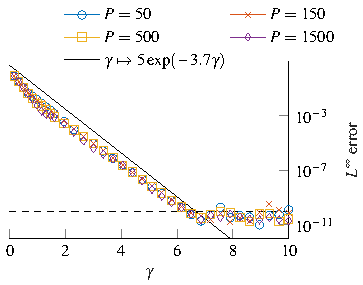
\includegraphics[scale = 0.7]{EBD/figs/ApplicationNumLaplace}			
	\caption{Evolution of the $L^{\infty}$ error over $[a,1]$ associated to the EBD for different values of $P$ in function of $\Pa$. An exponential decay is indeed observed at the roughly estimated rate of $\propto \exp(-3.7\Pa)$. The error stops decreasing at $e_{\min} \approx 10^{-10}$, for a value of $\Pa \approx 6.7$ because of the ill conditioning of the linear system \eqref{LinearSystem}}
	\label{ApplicationNumLaplace}
\end{figure}

\subsection{Helmholtz kernel}
\label{HelmoholtzSubSection}
Let $Y_0$ the classical Bessel function of second kind and of order $0$. For any frequency number $k>0$, the Helmholtz kernel, $r \mapsto \frac{-i}{4}H^{(1)}_0(kr)$, where $H^{(1)}_0(r) = J_0(r) + i Y_0(r)$, is the Green kernel associated to the harmonic wave operator $- \Delta - k^2$, that satisfies a Sommerfeld radiation condition at infinity. This kernel arises in various physical problems such as sound waves scattering  (see for example  \cite{wilcox1975scattering}). To approximate $H^{(1)}_0(kr)$ as a sum of dilated $J_0$ functions, it is sufficient to study the function of $r \mapsto Y_0(kr)$. We now have three different cases:
\begin{itemize}
	\item[-]\textbf{When $k$ is a root of $Y_0$}: In this case the multi-Dirichlet condition is satisfied at any order. Indeed, for any $n$, 
	\[(-\Delta)^n Y_0(kr)\big|_{r=1} = k^{2n} Y_0(k) = 0\,.\]
	We thus compute the EBD decomposition of $Y_0$ on an interval $(a,1)$. 
	\item[-]\textbf{When $k$ is greater than the first root of $Y_0$}: we compute the EBD for $r \mapsto Y_0(k'r)$ on $(a,1)$, where $k'$ is the smallest root of $Y_0$ greater than $k$. This provides a decomposition for $r \mapsto Y_0(kr)$ valid on $(\frac{k'}{k}a,\frac{k'}{k})$.
	\item[-]\textbf{When $k$ is much smaller than the first root of $Y_0$}: Here, instead of rescaling, one can use the Bessel-Fourier series associated to the Robin condition (see \autoref{Robin}):
	\[\dfrac{\partial u}{\partial n} + H u = 0\,,\]
	with $H = -\dfrac{k Y_0'(k)}{Y_0(k)} > 0$ in this region. 
\end{itemize}
\noindent

\subsection{General kernel : enforcing the multi-Dirichlet condition}
\label{begal1}
For a general radial kernel $G$, the multi-Dirichlet conditions may not be fulfilled. When applying the EBD method without any changes, this leads to errors near $r=1$. In this case, we apply the EBD to a modified function $H = G - K$ where $K$ is chosen to enforce the multi-Dirichlet condition. We can take for example
\[K(r) = \sum_{t=1}^{n} \mu_t J_0(\omega_t r)\,,\]
where $\omega_1$ is the root of $J_1$ that is closest from the ratio $\sqrt{\abs{\frac{G(1)}{\Delta G(1)}}}$ and $\omega_2, \cdots, \omega_n$, are the subsequent roots of $J_1$. The coefficients $(\mu_t)_{1 \leq t \leq n}$ are found by solving
\[M\mu = \lambda\,,\]
where $\lambda$ is the vector given by
\begin{eqnarray*}
	\lambda_t &=& (-\Delta)^t G \big|_{r=1}\,, \quad t\in \{1,\cdots,n\}\,,
\end{eqnarray*}
and
\[M=
\begin{bmatrix}
-\omega_1^2          & -\omega_2^2          & \cdots & -\omega_n^2          \\
\vdots               & \vdots               & \cdots & \vdots               \\
(-1)^n \omega_1^{2n} & (-1)^n \omega_2^{2n} & \cdots & (-1)^n \omega_n^{2n} \\ 
\end{bmatrix}.
\]
\vspace{5pt}

In \autoref{figArbitraryKernel}, we show the efficiency of this method by applying the EBD with $100$ terms to some highly oscillating function ($x \mapsto \log(x) + \sin(250x)$) and computing the maximal error of the decomposition in function of the parameter $\gamma = Pa$ (recall $P$ is the number of terms in the Bessel decomposition and $a$ is the inner radius of the annulus of approximation). We choose the frequencies $\varInRange{\omega}{t}{1}{n}$ as the roots of $J_1$ that are closest to $250$. This figure illustrates the importance of the multi-Dirichlet condition for the fast decay of the error. 

\begin{figure}[t]	
	\centering
	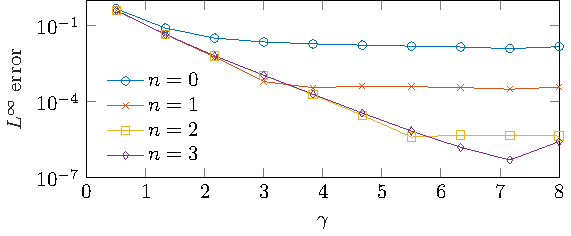
\includegraphics[scale = 0.8]{EBD/figs/LinfVsGamma_arbitraryKern}
	\caption{Maximal error between the kernel $G_1(r) =  \log(x) + \sin(250x)$ and its $100$-terms EBD in function of $\gamma = Pa$ using the method described in this paragraph for several values of $n$. Without any change to the method ($n = 0$) the $L^\infty$ error stops decreasing after some value of $\gamma$. Enforcing the multi-Dirichlet condition to higher order gradually improves the maximal reachable accuracy}
	\label{figArbitraryKernel}
\end{figure}																									

\section{Circular quadrature}
\label{sec:circular}
In this section, we study the approximation
\[ J_0(\rho_p|x|) \approx \dfrac{1}{M_p}\sum_{m=0}^{M_p-1}e^{i \rho_p \bs{\xi}^p_m \cdot x}\,, \]
where $M_p$ is an integer and with
\begin{equation}
\label{defXimp}
\xi_m^p = \left(\cos\left(\frac{2 m \pi}{M_p}\right),\sin\left(\frac{2 m\pi }{M_p}\right)\right)\,, \quad 0 \leq m \leq M_p - 1\,.
\end{equation} 
This approximation is obtained by applying the trapezoidal rule to the identity 
\[ J_0(|x|) = \int_{\partial B} e^{i x \cdot \xi} d\xi\,.\]
\begin{remark}
	In the SCSD method, the Bessel functions are replaced by cardinal sines because
	\[ \sinc(\abs{\bs{x}}) =  \frac{1}{4\pi}\int_{\abs{\bs{\xi}}=1} e^{i \bs{x}\cdot \bs{\xi}} d\sigma(\bs{\xi}) \,, \]
	where the integral is now taken over $\mathbb {S}^2 \subset \R^3$. 
\end{remark}
\begin{theorem} There exists a constant $K$ such that for any $r>0$, for any integer $M \geq \frac{e}{2}r$, and for any $\varphi \in \R$ 
	\[\left|J_0(r) -  \dfrac{1}{M}\sum_{m=0}^{M-1}e^{ir\sin\left(\frac{2m\pi}{M}-\varphi\right)} \right| \leq K \left(\dfrac{er}{2M}\right)^M\,.\]
	\label{QuadratureCirc}
\end{theorem}
\begin{proof}
	Let $f : x \mapsto e^{ir\sin(x - \varphi)}$. For any $k \in \Z$, one has
	\[J_k(r) =  \int_{0}^{2\pi}e^{ir\sin(x)}e^{-ikx}dx =  e^{-ik\varphi}\int_{0}^{2\pi}f(x)e^{-ikx}dx\,.\] 
	Thus, the (usual) Fourier coefficient of $f$ are given by 
	\[c_k(f) = e^{ik\varphi}J_k(r).\]
	Consequently, the aliasing formula yields 
	\[J_0(r) -  \dfrac{1}{M} \sum_{j=0}^{M-1} e^{ir \sin \left( \frac{2j\pi}{M}-\varphi \right)} = -\sum_{k\in \Z^*}e^{iNk\varphi}J_{Nk}(r)\,.\] 
	For large $\abs{k}$, we have
	\[J_k(r) \sim \left(\dfrac{er}{2\abs{k}}\right)^{\abs{k}}\,.\]
	Therefore, there exists a constant $C'$ such that: 
	\begin{eqnarray*}
		\abs{J_0(r) -  \dfrac{1}{M}\sum_{m=0}^{M-1}e^{ir\sin\left(\frac{2m\pi}{M}-\varphi\right)}} &\leq& C' \sum_{k\in \Z^*} \left(\dfrac{er}{2M|k|}\right)^{M|k|}\\
		&\leq& K \left(\dfrac{er}{2M}\right)^M 
	\end{eqnarray*}
	for an appropriate choice of $K$.	
	\qed
\end{proof}
We conclude with the following result
\begin{proposition} Let $\varepsilon >0$, $r>0$, and assume $M > \dfrac{e}{2}r + \log\left(\dfrac{K}{\varepsilon}\right)$. Then 
	\[\left|J_0(r) -  \dfrac{1}{M}\sum_{m=0}^{M-1}e^{ir\sin\left(\frac{2m\pi}{M}-\varphi\right)} \right| \leq \varepsilon\,.\]
	\label{suboptCirc}
\end{proposition}
\begin{proof}
	This results from \autoref{QuadratureCirc} and the following inequality:
	\[ \forall (A,B) \in \left(\mathbb{R}_+^*\right)^2, \quad  \left( \dfrac{A}{A+B}\right)^{A+B} \leq e^{-B}\,.\]
	which may be proved using $\left(1+x^{-1}\right)\log(1+x) \geq 1$ valid for all $x \neq 0$. 
	\qed
\end{proof}
Our numerical tests suggest that the constant $\frac{e}{2}$ in the previous estimation is sharp. 


\section{Proof of the complexity}
\label{sec:complexities}
We now sum up all the results obtained in the previous sections to prove the complexity of the complete algorithm given in \autoref{sec:overview}. We fix a free parameter $\eta \in [0,1/6]$ and choose the inner radius of the annulus of approximation as
\begin{equation}
\label{def_a}
a = \dfrac{1}{N_z^{2/3 - \eta}}\,.
\end{equation}  
We give a bound for the number of operations in function of the number of nodes $N_z$, the target tolerance $\varepsilon$ and $\eta$. Let  $C_{\textup{EBD}}$, $C_{\textup{circ}}$, $C_{\textup{assemble}}$, $C_{\textup{far}}$ and $C_{\textup{close}}$ respectively denote the number of operations required  to compute the EBD, the circular quadrature, to assemble the close correction matrix $D$ \eqref{defD}, to compute the far approximation \eqref{FarApprox}, and to apply $D$ on a vector. In the sequel, $C$ is used for any positive constant that is independent of $N_z$, $\varepsilon$ and $\eta$. 
\subsection{Offline computations}
\subsubsection{Trigonometric representation}	
Recall that we compute a trigonometric representation of the form \eqref{Gapprox} for the kernel $G(r) =\log(r)$, by first computing its EBD:
\[ G(x) \approx \sum_{p=1}^P \alpha_p e_p(x)\,,\]
where $e_p(r) = C_p J_0(\rho_p r)$ are the normalized eigenfunctions of the Laplace operator and the number of terms $P$ is chosen large enough so that the $L^\infty$ error is below the required tolerance. In a second step, each function $e_p$ is replaced by the circular quadrature analyzed in \autoref{sec:circular}. 
\paragraph{Efficient Bessel Decomposition.}
If the EBD is applied on the annulus $\{a < r < 1\}$, \autoref{theRadialQuadLaplaceErreur} shows that the tolerance $\frac{\varepsilon}{2}$ is reached for 
\begin{equation}
\label{eq:valeurDePenFonctionDe_a}
P = O\left(\dfrac{|\log(\varepsilon)|}{a}\right)\,.
\end{equation}
Since the coefficients are obtained through the inversion of a $P \times P$ matrix, the computation of the EBD requires $O(P^3)$ computations. Therefore, with $a$ defined as in \eqref{def_a}, one has
\begin{equation}
\label{Complex:EBD}
C_{\textup{EBD}}(N_z,\varepsilon,\eta) \leq C \abs{\log\varepsilon}^3 N_z^{2 - 3\eta}\,.
\end{equation}

\paragraph{Circular quadrature.} Using the notation of \autoref{sec:circular}, we choose the number $M_p$ of terms in the circular quadrature for each $e_p$ such that
\begin{equation}
\label{temp1}
\abs{e_p(|x|) - \dfrac{C_p}{M_p}\sum_{m=1}^{M_p} e^{i \rho_p \bs{x} \cdot \bs{\xi}_m^p}} \leq \frac{\varepsilon}{2P \abs{\alpha_p}} \quad a < \abs{\bs{x}} < 1\,.
\end{equation}
By the triangle inequality, this ensures that the maximal error in the trigonometric representation of $G$ is less than $\varepsilon$. According to  \autoref{suboptCirc}, we may choose $M_p$ such that
\begin{equation}
M_p > \frac{e}{2} \rho_p + \log\left(\dfrac{2KP |\alpha_p|C_p}{\varepsilon}\right).
\end{equation} 
Bessel's identity ensures the boundedness of $\alpha_p$, and the constants $C_p$ are bounded by estimation \eqref{estimCp}. Since $\rho_p = O(p)$, the total number of terms  $N_\xi$  in the trigonometric representation is of the order
\begin{equation}
\label{eq:NxiEnFonctionDeP}
N_\xi = \sum_{p = 1}^P M_p = O(P^2)
\end{equation}
and $C_\text{circ}(N_z,\varepsilon,\eta) \leq C \abs{\log\varepsilon}^2 N_z^{4/3 - 2\eta}$. We thus see that the EBD dominates the complexity for computing the trigonometric representation, and the estimation \eqref{Complex:EBD} yields the first part of \autoref{The:GlobalComplexity}.

\subsubsection{Close correction matrix:} 
Recall that $\rmax$ is the diameter of the cloud of nodes $(z_k)$. 
Fix $\rmin \isdef a \rmax$. We first determine the set $\mathcal{P}$ of all pairs $(k,l)$ such that $\abs{\bs{z}_k - \bs{z}_l} \leq \delta_{\min}$. This is the classical "fixed-radius near neighbors search", and can be solved in $O(N_z \log N_z + \# \mathcal{P})$ operations (see for example \cite{bentley1975multidimensional, bentley1977complexity,turau1991fixed,dickerson1990fixed}). In order to compute the close correction sparse matrix:
\[
D_{kl} = \delta_{(k,l) \in \mathcal{P}} \left( G({\bs{z}_k - \bs{z}_l}) - \sum_{p = 1}^{P} \alpha_p J_0\left(\frac{\rho_p}{\rmax} |\bs{z}_k - \bs{z}_l|\right)\right)\,,
\]
we need $\#\mathcal{P}$ evaluations of $\log$. For the computation of the second term, we use a piecewise polynomial interpolation of the smooth function.
\[f: r \mapsto \sum_{p = 1}^{P} \alpha_p J_0(\rho_pr)\,, \quad r \in (0,a)\,.\]
This involves only a small number of interpolation nodes, and the sum can be evaluated in $O(N_z)$ operations. For a set of nodes uniformly distributed on a curve, we have
\begin{equation}
\label{eq:NombreDinteractionsProches}
\# \mathcal{P} = O\left(\dfrac{\rmin}{\rmax} N_z\right) = O(N_z^2 a)\,.
\end{equation}
We thus get
\begin{equation}
\label{Complex:assemble}
C_{\textup{close}}(N_z,\varepsilon,\eta) \leq C N_z^{4/3 + \eta}\,.
\end{equation}
This is the second part of \autoref{The:GlobalComplexity}. 
\subsection{Online Computations}
\paragraph{Far approximation.} Recall that for all $k \in \{1,\cdots,N_z\}$, the far approximation is defined by the following equation:
\[ q^{\text{far}}_k = \sum_{l=1}^{N_z} G_{\textup{trig}}(\bs{z}_k - \bs{z}_l) f_l,\]
where
\[ G_{\textup{trig}}(\bs{x}) = \sum_{\nu=1}^{N_\xi} \hat{\omega}_\nu e^{i \bs{x} \cdot \bs{\xi}_\nu}.\]
To compute $q^{\textup{far}}$, recall the following three steps:
\begin{itemize}
	\setlength{\itemindent}{2em}
	\item[(i)] \textbf{Space $\rightarrow$ Fourier: } Compute $\hat{f} = \textup{NUFFT}_-[\bs{z},\boldsymbol{\xi}](f),$
	\item[(ii)] \textbf{Fourier multiply} Perform element wise multiplication by $\hat{\omega}$: 
	\[\hat{g}_{\nu} = \hat{\omega}_\nu \hat{f_\nu},\]
	\item[(iii)] \textbf{Fourier $\rightarrow$ Space: } Compute $q^{\text{far}} =  \textup{NUFFT}_+[\bs{z},\boldsymbol{\xi}](\hat{g}).$
	\setlength{\itemindent}{0em}
\end{itemize}
According to \cite[Sec.	 4.3]{keiner2009using}, the complexity of the NUFFT of type 3 is 
\[O\left(B_1 B_2 \log (B_1 B_2) + \abs{\log\varepsilon}^2(N_x + N_\xi)\right)\]
where $B_1$ and $B_2$ are the bandwidth parameters along each dimension. Here all frequencies lie in a circle of radius $\rho_P = O(P)$, thus $B_1B_2 = O(P^2)$. On the other hand, equations \eqref{def_a} and  \eqref{eq:NxiEnFonctionDeP} imply that $N_{\xi} \geq N_z$, and by \eqref{eq:NxiEnFonctionDeP}, $N_\xi = O(P^2)$. Therefore, the complexity of the NUFFT is $O(P^2 \log(P) \abs{\log \varepsilon}^2)$. By definition \eqref{def_a} and eq. \eqref{eq:valeurDePenFonctionDe_a}, we conclude
\begin{equation}
\label{Complex:far}
C_{\textup{far}}(N_z,\varepsilon,\eta) \leq C N_z^{4/3 - 2\eta}\log(N_z) \abs{\log \varepsilon}^{4} .
\end{equation}
\paragraph{Close correction.} Since $D$ has $\# \mathcal{P}$ non-zero entries, we get 
\begin{equation}
\label{Complex:close}
C_{\textup{close}}(N_z,\varepsilon,\eta) \leq C N_z^{4/3 + \eta}.
\end{equation}
Summing \eqref{Complex:far} and \eqref{Complex:close} yields the second part of \autoref{The:GlobalComplexity}. 

\begin{remark}
	The extreme cases $\eta= 0$ and $\eta = 1/6$ correspond respectively to the situations where one wishes to either minimize the total (offline $+$ online) computation time or just the online time. The corresponding complexities are given in the table below (omitting the dependence in $\varepsilon$):	
	\begin{table}[H]
		\centering
		\begin{tabular}{ |c|c|c| } 
			\hline
			& $\eta = 0 $    & $\eta = 1/6$       \\ 
			\hline
			Offline   & $O(N_z^2)$  & $O\left(N_z^{3/2} \log N_z\right)$  \\ 
			Online & $O(N_z^{4/3} \log(N_z))$ & $O(N_z^{3/2})$ \\ 
			\hline
		\end{tabular}
		\caption{Complexity of the algorithm (omitting dependence in $\varepsilon$) in the two extreme cases $\eta=0$ and $\eta = 1/6$.}
	\end{table}									
\end{remark}

\section{Performance of the method and comparison with \textit{Fastsum}}
\label{sec:numericalPerf}
In this section, we apply our method (which we call EBD) to compute the vector $q$ given by 
\[q_k = \sum_{l = 1}^{N} G(X_k - Y_l) f_l, \quad k = 1, \cdots, N\]
where $X$ and $Y$ are two distinct clouds of points in $\R^2$ of size $N$. The performance is compared with \textit{Fastsum}, which sources are downloaded from the toolbox \cite{Fastsum}. We study three kernels, $G_1(x) = \log(x)$, $G_2(x) = x^2 \log(x)$ and $G_3(x) = \frac{1}{x^2}$. We measure the computing times for $N$ from $10^3$ to $10^6$. The computer used for these tests is a laptop cadenced to 1.6 GHz and possessing 4GB of memory.

We measure the "offline" time as the time needed to set up the method and compute the first discrete convolution. The "online" time is the average time needed for the subsequent convolutions. 

\paragraph{Parameter setting.}
For \textit{Fastsum}, we use the parameter setting described in \cite{potts2004fast} for singular kernels. For the first two kernels, we use the cut-off parameter $m= 4$ and the degree of regularization $p = 3$. The approximate error level $\varepsilon$ is measured by computing the maximal absolute error between $G(X_1 - Y_l)$ and its approximation by the trigonometric polynomial for $l = 1, \cdots, N$. This is taken as the (input) target tolerance in the EBD. For the third kernel, it is necessary to increase $m$ and $p$ in \textit{Fastsum} to obtain an acceptable error. In such case, we take $p = m$ and choose the first value for which the error goes below $1$. In our algorithm, the only free parameter is the inner radius of the annulus of approximation $\rmin$. Depending on the case, we set $\rmin = \frac{\lambda}{\sqrt{N}} \rmax$ with $\lambda$ ranging from $2$ to $20$. 

\paragraph{Programming language.}
Our program is written in Matlab except for the NUFFT routine which is the FORTRAN routine borrowed from the NYU website \cite{NUFFTGg}. In contrast, Fastsum is fully written in C. This difference only plays a role in the offline computations, since in the online stage, most of the time is spent in the NUFFT for both methods. 
\paragraph{Discussion.}
We observe that our method yields a representation of the radial kernel with much less frequency samples (a factor $100$ is observed in most cases). The offline computations for EBD are always longer (by a factor $2$ to $4$ in computational intensive cases). After that, our method is faster than \textit{Fastsum} for evaluating the convolution in every case, in general by a factor $2$ to $3$. This gain in online performance for EBD is particularly useful when one wishes to solve iteratively a large linear system with matrix entries of the form $G(X_k - Y_l)$. 

In our algorithm, the 1D approximation allows for an accurate estimation of the error which can therefore be given and controlled as an input. Instead, in \textit{Fastsum}, the parameters need a fine tuning "by hand" in order to achieve a given accuracy. 

On the other hand, there is a free parameter in the EBD method, $\rmin$, that determines the performance. When the distribution of the nodes is known, the above analysis provides a way to select $\rmin$ to ensure a quasi-linear complexity. However, it is not clear how to choose the optimal value for $\rmin$ automatically when the distribution of nodes is not known. 

\begin{table}[H]
	\centering
	\caption{Computing times (s) for the kernel $G(x) = \log(x)$}
	\begin{tabular}{*9c}
		\toprule
		&  \multicolumn{4}{c}{\textit{Fastsum}} & \multicolumn{4}{c}{EBD}\\
		\cmidrule(lr){2-5}\cmidrule(lr){6-9}
		$N$   & $N_\xi$ & Offline   & Online    & $\varepsilon$ & $N_\xi$ & Offline   & Online  & $\varepsilon$ \\
		$10^3$   & $1.2$e4 & $2.1$e-2   & $5.7$e-3    & $1.3$e-3 & $150$ & $0.31$   & $2.0$e-3  & $1$e-3 \\
		$10^4$   & $1.2$e5 & $0.14$   & $7.3$e-2    & $1.3$e-3 & $2.4$e3 & $0.7$  & $1.3$e-2 & $1.2$e-3 \\
		$10^5$   & $1.2$e6 & $1.4$ & $0.9$    & $1.3$e-3 & $2.8$e4 & $3.8$   & $0.15$  & $1.2$e-3 \\
		$10^6$   & $1.2$e7 & $16$   &  $10$    & $1.3$e-3 & $1.2$e6 & $30$ & $4.6$  & $1.3$e-3 \\
		\bottomrule
	\end{tabular}
\end{table}
\vspace{-0.5cm}
\begin{table}[t]
	\centering
	\caption{Computing times (s) for the kernel $G(x) = x^2\log(x)$}
	\begin{tabular}{*9c}
		\toprule
		&  \multicolumn{4}{c}{\textit{Fastsum}} & \multicolumn{4}{c}{EBD}\\
		\cmidrule(lr){2-5}\cmidrule(lr){6-9}
		$N$   & $N_\xi$ & Offline   & Online    & $\varepsilon$ & $N_\xi$ & Offline   & Online  & $\varepsilon$ \\
		$10^3$   & $1.3$e4 & $2.2$e-$2$   & $5.9$e-$3$    & $1$e-5 & 166 & 0.92   & $2.6$e-$3$   & $6.3$e-6 \\
		$10^4$   & $1.2$e5 & $0.15$  & $7.4$e-2    & $7.6$e-7 & $1.7$e3 & $0.94$   & $2.5$e-2  & $5.3$e-7 \\
		$10^5$   & $1.2$e6 & $1.5$   & $0.91$    & $2.1$e-8 & $3.2$e4 & $3.8$   & $0.35$  & $2$e-8 \\
		$10^6$   & $1.2$e7 & $16$   & $10$    & $1.5$e8 & $3.7$e5 & $28$   & $8$  & $1.5$e8 \\		
		\bottomrule
	\end{tabular}
\end{table}

\begin{table}[t]
	\centering
	\caption{Computing times (s) for the kernel $G(x) = \frac{1}{x^2}$}
	\begin{tabular}{*9c}
		\toprule
		&  \multicolumn{4}{c}{\textit{Fastsum}} & \multicolumn{4}{c}{EBD}\\
		\cmidrule(lr){2-5}\cmidrule(lr){6-9}
		$N$   & $N_\xi$ & Offline   & Online    & $\varepsilon$ & $N_\xi$ & Offline   & Online  & $\varepsilon$ \\
		$10^3$   &  $2.1$e4 &  $2.5$e-2  & $7$e-3  & $6$e-2 & $1.5$e2 & $ 0.45$ & $1.8$e-3 & $5$e-2 \\
		$10^4$   & $2.4$e5 & $0.23$ & $0.12$  & $0.17$ 
		& $5.2$e3 & $1.2$ & $1.65$e-2 & $0.14$\\
		$10^5$  &  $2.8$e6 & $3$  & $1.5$  & $0.2$ & 
		$1.5$e5 & $7.8$ & $0.36$ & $0.2$\\
		$10^6$ & $3.2$e7  & $45$ & $25$  & 0.6& 
		$5.2$e6  & $145$ & $16.5$ & $0.5$\\
		\bottomrule
	\end{tabular}
\end{table}
\subsection*{Conclusion}
The method that we have presented (EBD) generalizes the SCSD method of \cite{Alouges2015} from $3$ to $2$ dimensions. Compared to SCSD, the cardinal sines must be replaced by Bessel functions, and the Fourier series appearing in 3D become Fourier-Bessel series in 2D. We have provided a complete analysis of the complexity and the error of our method. It is shown that the computational complexity is quasi-linear in terms of the number of nodes. We also provide numerical results that confirm the theoretical estimations. It has appeared that the structure of SCSD and EBD is very similar to that of \textit{Fastsum}, differing only by the choice of the frequency samples. By exploiting the radial symmetry, our method allows to reduce drastically the number of those samples. As a result, after some precomputations, the EBD yields faster approximations of the discrete convolutions than \textit{Fastsum}. Future work includes generalizing the present approach to $n$ dimensions, and the automatic fine-tuning of the remaining free parameter of the method, $\rmin$.

\bibliographystyle{plain}
\bibliography{EBD/Biblio/biblio}

\end{document}